%%%%%%%%%%%%%%%%%%%%%%%%%%%%%%%%%%%%%%%%%
% NIWeek 2014 Poster by T. Reveyrand
% www.microwave.fr
% http://www.microwave.fr/LaTeX.html
% ---------------------------------------
% 
% Original template created by:
% Brian Amberg (baposter@brian-amberg.de)
%
% This template has been downloaded from:
% http://www.LaTeXTemplates.com
%
% License:
% CC BY-NC-SA 3.0 (http://creativecommons.org/licenses/by-nc-sa/3.0/)
%
%%%%%%%%%%%%%%%%%%%%%%%%%%%%%%%%%%%%%%%%%

%----------------------------------------------------------------------------------------
%	PACKAGES AND OTHER DOCUMENT CONFIGURATIONS
%----------------------------------------------------------------------------------------

\documentclass[a0paper,portrait]{baposter}

\usepackage[font=small,labelfont=bf]{caption} % Required for specifying captions to tables and figures
\usepackage{booktabs} % Horizontal rules in tables
\usepackage{relsize} % Used for making text smaller in some places

\usepackage{amsmath, amsfonts, amssymb, amsthm} % Math packages
\usepackage{eqparbox}

\usepackage{textcomp}

\usepackage{hyperref}

\graphicspath{{images/}} % Directory in which figures are stored

 \definecolor{bordercol}{RGB}{40,40,40} % Border color of content boxes
 \definecolor{headercol1}{RGB}{186,215,230} % Background color for the header in the content boxes (left side)
 \definecolor{headercol2}{RGB}{120,120,120} % Background color for the header in the content boxes (right side)
 \definecolor{headerfontcol}{RGB}{0,0,0} % Text color for the header text in the content boxes
 \definecolor{boxcolor}{RGB}{210,235,250} % Background color for the content in the content boxes
 
\definecolor{jdhblue}{RGB}{2,93,186}

\definecolor{zkblue}{RGB}{88,135,175}
\definecolor{zkbackground}{RGB}{230,232,234}


\usetikzlibrary{shapes, arrows, external, decorations.pathmorphing, backgrounds, positioning, fit, petri, calc, hobby, cd}


\begin{document}

% \background{ % Set the background to an image (background.pdf)
% \begin{tikzpicture}[remember picture,overlay]
% \draw (current page.north west)+(-2em,2em) node[anchor=north west]
% {\includegraphics[height=1.1\textheight]{images/baposter_background.pdf}};
% \end{tikzpicture}
% }

\begin{poster}{
grid=false,
borderColor=bordercol, % Border color of content boxes
headerColorOne=headercol1, % Background color for the header in the content boxes (left side)
headerColorTwo=headercol2, % Background color for the header in the content boxes (right side)
headerFontColor=headerfontcol, % Text color for the header text in the content boxes
% boxColorOne=boxcolor, % Background color for the content in the content boxes
boxColorOne=zkbackground,
headershape=roundedright, % Specify the rounded corner in the content box headers
headerfont=\Large\sf\bf, % Font modifiers for the text in the content box headers
textborder=rectangle,
% background=user,
background=none,
headerborder=open, % Change to closed for a line under the content box headers
boxshade=plain
}
%
%----------------------------------------------------------------------------------------
%	TITLE AND AUTHOR NAME
%----------------------------------------------------------------------------------------
%
{
\includegraphics[scale=0.101]{logo_tmu.jpeg}} % University/lab logo
{
% {\bf \fontsize{19pt}{19pt} \selectfont Searching for Effective Neural Network Architectures} \\
% {\it \LARGE  for Heart Murmur Detection from Phonocardiogram}
% } % Poster title
{\bf \fontsize{19pt}{19pt} \selectfont Predicting Neurological Recovery from Coma with Longitudinal EEG Using Deep Neural Networks}
} % Poster title
{\vspace{0.3em} \smaller Jingsu KANG$^1$, Hao WEN$^2$  \\  % Author names

$^1${\it Tianjin Medical University}\qquad
$^2${\it College of Science, China Agricultural University} \\
\vspace{0.2cm}
{\Large \bf{The George B. Moody PhysioNet Challenge 2023}, ~~~\bf{Team Revenger}}
}
{
\includegraphics[scale=0.401]{images/logo_cau_science.png}}


\newif\ifcoloredtext
\coloredtexttrue
\newif\ifboxednn
\boxednntrue


%----------------------------------------------------------------------------------------
%	INTRODUCTION
%----------------------------------------------------------------------------------------

\headerbox{Introduction}{name=introduction, column=0, row=0, span=3}{
% finished

\begin{itemize}
\item We modelled the problem as a \textbf{classification problem} where the learning objective is the discrete CPC scores (1 - 5). The final clinical outcome prediction is obtained via the mapping: CPC = 1 or 2 $\to$ ``Good outcome''; CPC = 3, 4, or 5 $\to$ ``Poor outcome''.
\vspace{-0.2cm}
\item Offline signal quality index (SQI) was computed offline for EEG recordings. A part of EEGs was selected for training based on SQI.
\vspace{-0.2cm}
\item We used a \textbf{time-incremental convolutional recurrent neural network (TiCRNN model} to make per-recording probability vectors, which were averaged and re-normalized via \texttt{Softmax} to obtain per-patient predictions from multiple EEG recordings.
\end{itemize}
}


%----------------------------------------------------------------------------------------
%	NN architecture
%----------------------------------------------------------------------------------------

\headerbox{Main Model: TiCRNN}{name=nn, column=0, span=1, row=1, below=introduction}{
% finished

% finished

\begin{tikzpicture}%[node distance = 1cm, auto]

% \tikzstyle{block} = [rectangle, draw, text width = 5em, text centered, rounded corners, inner sep = 3pt, minimum height = 1.0em]

\tikzstyle{wideblock} = [rectangle, draw, text width = 12em, text centered, rounded corners, inner sep = 3pt, minimum height = 1.0em]

\pgfmathsetmacro\blockdist {0.4}
\pgfmathsetmacro\pathshift {0.1}

\node [rectangle, text width = 12em, text centered, rounded corners, inner sep = 3pt, minimum height = 1.0em] (input) {EEG Waveform};

\node [wideblock, below = \blockdist of input] (stem) {Stem Conv};
\path[->] ([yshift = -\pathshift]input.south) edge ([yshift = \pathshift]stem.north);

\ifcoloredtext
\node [wideblock, below = \blockdist of stem] (bottleneck) {\bf\color{red}4 $\times$ SE-Bottleneck};
\path[->] ([yshift = -\pathshift]stem.south) edge ([yshift = \pathshift]bottleneck.north);
\else
\node [wideblock, below = \blockdist of stem] (bottleneck) {\bf 4 $\times$ SE-Bottleneck};
\path[->] ([yshift = -\pathshift]stem.south) edge ([yshift = \pathshift]bottleneck.north);
\fi

\node [wideblock, below = \blockdist of bottleneck] (lstm) {2 $\times$ Bidirectional LSTM};
\path[->] ([yshift = -\pathshift]bottleneck.south) edge ([yshift = \pathshift]lstm.north);

\node [wideblock, below = \blockdist of lstm] (se) {SE Global Attention};
\path[->] ([yshift = -\pathshift]lstm.south) edge ([yshift = \pathshift]se.north);

\node [wideblock, below = \blockdist of se] (pool) {Adaptive Average Pooling};
\path[->] ([yshift = -\pathshift]se.south) edge ([yshift = \pathshift]pool.north);

\node [wideblock, below = \blockdist of pool] (mlp) {Multi-Layer Perceptron};
\path[->] ([yshift = -\pathshift]pool.south) edge ([yshift = \pathshift]mlp.north);

\node [rectangle, text width = 12em, text centered, rounded corners, inner sep = 3pt, minimum height = 1.0em, below = \blockdist of mlp] (prob) {Probability Vectors for 5 CPC Scores};
\path[->] ([yshift = -\pathshift]mlp.south) edge ([yshift = \pathshift]prob.north);

\draw[rounded corners, dashed, thick] ([xshift = -80, yshift = -5]mlp.south) rectangle ([xshift = 80, yshift = 5]stem.north);
\ifboxednn
\draw[rounded corners, ultra thick] ([xshift = -103, yshift = -5]prob.south) rectangle ([xshift = 103, yshift = 5]input.north);
\fi

\end{tikzpicture}


We used a {\color{red}T}ime-{\color{red}i}ncremental {\color{red}C}onvolutional {\color{red}R}ecurrent {\color{red}N}eural {\color{red}N}etwork ({\color{red}TiCRNN}) model to predict CPC scores for the EEG recordings.

}
\headerbox{Neural Network Backbone}{name=backbone, column=1, span=2, row=1, below=introduction}{
% finished

\begin{figure}
\centering

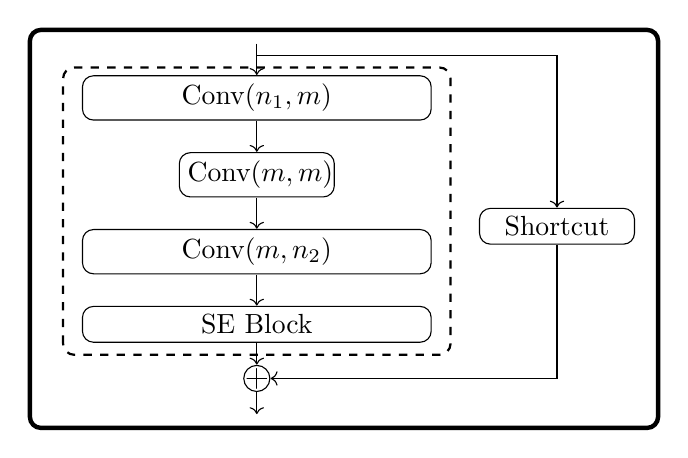
\begin{tikzpicture}%[node distance = 1cm, auto]

\tikzstyle{block} = [rectangle, draw, text width = 5em, text centered, rounded corners, inner sep = 3pt, minimum height = 1.0em]

\tikzstyle{wideblock} = [rectangle, draw, text width = 12em, text centered, rounded corners, inner sep = 3pt, minimum height = 1.0em]

\tikzset{%
  do path picture/.style={%
    path picture={%
      \pgfpointdiff{\pgfpointanchor{path picture bounding box}{south west}}%
        {\pgfpointanchor{path picture bounding box}{north east}}%
      \pgfgetlastxy\x\y%
      \tikzset{x=\x/2,y=\y/2}%
      #1
    }
  },
  plus/.style={do path picture={    
    \draw [line cap=round] (-3/4,0) -- (3/4,0) (0,-3/4) -- (0,3/4);
  }}
}

\coordinate (top) at (0, 0);
\pgfmathsetmacro\blockdist {0.4}
\pgfmathsetmacro\pathshift {0.1}

\node [wideblock, below = \blockdist of top] (conv1) {Conv($n_1, m)$};
\path [->] (top) edge ([yshift = \pathshift]conv1.north);

\node [block, below = \blockdist of conv1] (conv2) {Conv($m, m)$};
\path [->] ([yshift = -\pathshift]conv1.south) edge ([yshift = \pathshift]conv2.north);

\node [wideblock, below = \blockdist of conv2] (conv3) {Conv($m, n_2)$};
\path [->] ([yshift = -\pathshift]conv2.south) edge ([yshift = \pathshift]conv3.north);

\node [wideblock, below = \blockdist of conv3] (se) {SE Block};
\path [->] ([yshift = -\pathshift]conv3.south) edge ([yshift = \pathshift]se.north);

\node [circle, draw, plus, below = 0.7 * \blockdist of se] (plus) {};
\path [->] ([yshift = -\pathshift]se.south) edge ([yshift = \pathshift]plus.north);

\coordinate[below = 0.7 * \blockdist of plus] (bottom);
\path [->] ([yshift = -\pathshift]plus.south) edge (bottom);

\node [block, above right = -0.2 and 0.6 of conv3] (shortcut) {Shortcut};
\draw [->] ([yshift = 7]conv1.north) -| ([yshift = \pathshift]shortcut.north);
\draw [->] ([yshift = -\pathshift]shortcut.south) |- ([xshift = \pathshift]plus.east);


\draw[rounded corners, dashed, thick] ([xshift = -70, yshift = -11]se) rectangle ([xshift = 70, yshift = 11]conv1);
\draw[rounded corners, ultra thick] ([xshift = -82, yshift = -5]bottom) rectangle ([xshift = 145, yshift = 5]top);

\end{tikzpicture}

\caption{The structure of an SE-Bottleneck block. The mainstream in the dashed box consists of 3 convolutional blocks (actually compositions of convolution, batch normalization and activation) followed by an SE block. The channels $n_1, n_2$ are typically several times of $m,$ hence giving the name ``bottleneck''. The shortcut is typically convolutions of kernel size 1, whose stride and input/output channels match the mainstream.}
\label{fig:se_bottleneck}
\end{figure}
%
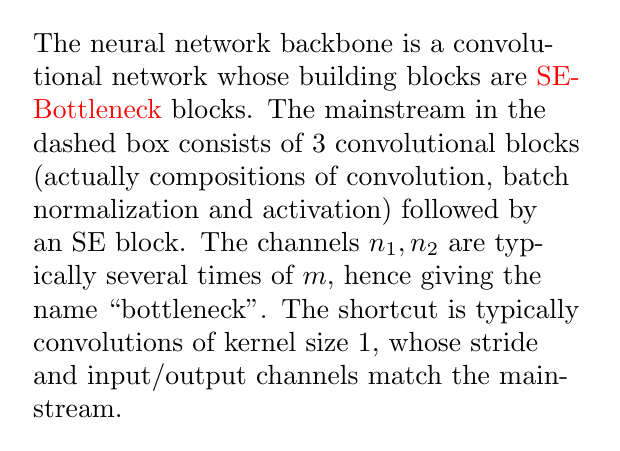
\begin{tikzpicture}
\node [rectangle, text width = 20em, inner sep = 2pt, minimum height = 1.0em] {The neural network backbone is a convolutional network whose building blocks are {\color{red}SE-Bottleneck} blocks. The mainstream in the dashed box consists of 3 convolutional blocks (actually compositions of convolution, batch normalization and activation) followed by an SE block. The channels $n_1, n_2$ are typically several times of $m,$ hence giving the name ``bottleneck''. The shortcut is typically convolutions of kernel size 1, whose stride and input/output channels match the mainstream.};
\end{tikzpicture}

}

%----------------------------------------------------------------------------------------
%	Preprocessing
%----------------------------------------------------------------------------------------

\headerbox{Preprocess Pipeline}{name=data, column=1, row=1, span=1, below=backbone}{
% finished
\begin{itemize}
    \item Butterworth bandpass filtering of order 4 and cutoff frequencies 0.5 - 30 Hz.
    \vspace{-0.2cm}
    \item Resampling to 100 Hz using polyphase filtering.
    \vspace{-0.2cm}
    \item Rescaling (Z-score normalization) to zero mean and unit variance.
\end{itemize}
}

%----------------------------------------------------------------------------------------
%	Training Setups
%----------------------------------------------------------------------------------------

\headerbox{Training Strategies}{name=training, span=1, column=2, row=1, below=backbone}{
% finished
\begin{itemize}
    \item Optimizer: AMSGrad variant of AdamW with OneCycleLR scheduler.
    \vspace{-0.2cm}
    \item Stratified train-validation split (split in patients): 80 \% -- 20 \%.
    \vspace{-0.2cm}
    \item Batch size 32; epoch number $\leq 55$ with early stopping patience 25 epochs.
\end{itemize}
}


%----------------------------------------------------------------------------------------
%	Submission Results
%----------------------------------------------------------------------------------------

% \headerbox{Submission Results}{name=submission, span=2, column=1, below=training}{
% % finished
% \begin{center}
% \begin{tabular}{r|c|c|c}
%     \hline
%     & \textbf{Murmur} & \multicolumn{2}{c}{\textbf{Outcome}} \\
%     & \textbf{weighted accuracy} & \multicolumn{1}{c}{\textbf{cost}} & \multicolumn{1}{c}{weighted accuracy} \\ \hline
%     Train & $0.88\pm 0.05$ & $8452\pm 2324$ & $0.88\pm 0.07$ \\
%     Train-val & $0.86\pm 0.01$ & $11341\pm 336$ & $0.79\pm 0.05$ \\ \hline
%     Hidden val & \textbf{0.689} & \textbf{9471.652} & NA \\
%     Ranking & \textbf{79/303} & \textbf{21/303} & NA \\ \hline
% \end{tabular}
% \end{center}
% Scores on the train, and train-val sets are provided with mean and standard deviation over most of our offline experiments. Scores on the hidden validation set are provided with the best scores out of the 10 submissions.
% }

%----------------------------------------------------------------------------------------
%	Limitations, Discussions
%----------------------------------------------------------------------------------------

% \headerbox{Discussions and Limitations}{name=discussion, column=0, below=dem, span=3}{
% % not finished
% \begin{itemize}
% \item Our multi-task learning (MTL) paradigm proved practical for the problems of heart murmur detection and clinical outcome identification from PCGs. The additional segmentation head makes the shared representation (the common backbone) learn more general features and thus improves the performances for the original two classification tasks the Challenge raised.
% \vspace{-0.2cm}
% \item All our models used \textbf{time-domain} signals, i.e. the \textbf{waveforms} as inputs. The derived \textbf{time-frequency-domain} signals, for example, the \textbf{spectrograms}, were not tested. Models that accept mixed-type inputs were not tested either.
% \vspace{-0.2cm}
% \item The need for Z-score normalization has to be reconsidered. More frequency-domain augmentation methods should be applied.
% \vspace{-0.2cm}
% \item The convolutional neural backbones proved effective, but still have room for improvement compared to top teams.
% \vspace{-0.2cm}
% \item The potential of models with the \textbf{transformer architecture} (e.g. the \textbf{wav2vec2} model) were not fully explored. As well as the powerfulness of model pretraining via self-supervised learning on larger datasets (e.g. the PhysioNet EPHNOGRAM dataset, etc.).
% \end{itemize}
% }


%----------------------------------------------------------------------------------------
%	REFERENCES
%----------------------------------------------------------------------------------------

%\headerbox{References}{name=references,column=2,below=application}{

%\smaller % Reduce the font size in this block
%\renewcommand{\section}[2]{\vskip 0.05em} % Get rid of the default "References" section title
%\nocite{*} % Insert publications even if they are not cited in the poster

%\bibliographystyle{unsrt}
%\bibliographystyle{IEEEtran}
%\bibliography{biblio} % Use biblio.bib as the bibliography file
%}


%----------------------------------------------------------------------------------------
%	ACKNOWLEDGEMENTS
%----------------------------------------------------------------------------------------

% \headerbox{Acknowledgements}{name=acknowledgements, column=0, below=discussion, span=3}{
% % finished
% % \smaller
% We would like to thank professor {\bf Deren Han} from the School of Mathematical Sciences, Beihang University and professor {\bf Wenjian Yu} from the Department of Computer Science and Technology, BNRist, Tsinghua University for generously providing GPU servers to help accomplish this work.

% \hfill \small \textit{Code, configs, etc. available at \href{https://github.com/DeepPSP/cinc2021}{https://github.com/DeepPSP/cinc2021}.}
% }

%----------------------------------------------------------------------------------------
%	link to the GitHub repository
%----------------------------------------------------------------------------------------

% \headerbox{}{name=foottext, column=0, span=3, below=acknowledgements, textborder=none, headerborder=none,  boxheaderheight=0pt}{
% % finished
% \hfill \small \textit{Code, configs, etc. available at https://github.com/DeepPSP/cinc2022}.
% }


\end{poster}

\end{document}
